\section{The min-plus map and the \texorpdfstring{$\sigma$}{sigma}-bump}
\label{sec:tropical}

Throughout this section the equation is \eqref{eq:familya}, with support
$S\subseteq\{1,\dots,k-1\}$ and $\theta$ as in the introduction; since the
numerator is nonzero, $S\ne\emptyset$ or $\theta=1$. The section sets up the
min-plus recursion and its leading coefficients (Theorems~\ref{thm:leading}
and~\ref{thm:P}), the tangent solutions that refute periodicity
(\autoref{thm:tangent}), and the $\sigma$-bump (\autoref{thm:sigmabump}). It
ends with a vocabulary for checking the conditions of a $\sigma$-bump
(\autoref{sec:nao-reading}) and the mirror lemma (\autoref{lem:nao-mirror}),
both used in the later sections.

\subsection{The min-plus recursion and its periodicity}
\label{sec:trop-minplus}

It is convenient to treat the constant term as a slot. Let
\[
S_\theta=S\cup\{0\}\ \text{if}\ \theta=1,\qquad S_\theta=S\ \text{if}\ \theta=0,
\]
so that $S_\theta\ne\emptyset$. For a sequence $(f_n)_{n\ge0}$ of real numbers, an index
$n\ge0$ and a slot $j\in S_\theta$, write
\[
v_n(f,j)=\begin{cases}0,&j=0,\\ f_{n+j},&j\in S,\end{cases}
\qquad
m_n(f)=\min_{j\in S_\theta}v_n(f,j).
\]
Thus $v_n(f,j)$ is the value read by slot $j$ from the window starting at $n$, and
the constant slot always reads $0$. The slots $j\in S$ are called \emph{taps}.

\begin{definition}
\label{def:trop-minplus}
An integer sequence $(e_n)_{n\ge0}$ is a \textit{solution of the min-plus
recursion} (for $k$, $S$, $\theta$) if
\begin{equation}
e_{n+k}+e_n=m_n(e)=\min\Bigl(\{0\ \text{if}\ \theta=1\}\cup\{e_{n+j}:j\in S\}\Bigr)
\qquad\text{for all}\ n\ge0.
\label{eq:trop-rec}
\end{equation}
Every integer window $(e_0,\dots,e_{k-1})$ extends uniquely to a solution. The
\textit{min-plus map} $T:\Z^k\to\Z^k$ is the corresponding window map,
$T(e_0,\dots,e_{k-1})=(e_1,\dots,e_{k-1},\,m_0(e)-e_0)$. The
\textit{attaining sets} of a solution $e$ are
\[
A_n=A_n(e)=\{\,j\in S_\theta:\ v_n(e,j)=m_n(e)\,\}\qquad(n\ge0);
\]
ties are allowed, so $A_n$ may have several elements.
\end{definition}

Each term of the orbit of \eqref{eq:familya} started from
$x_i=\delta^{e_i}$ behaves like $C_n\delta^{e_n}$ as $\delta\to0^+$, where the
exponents $e_n$ follow the min-plus recursion and the leading coefficients $C_n$
follow a recursion that keeps, in each step of \eqref{eq:familya}, only the
terms whose exponent attains the minimum.

\begin{theorem}[leading coefficients]
\label{thm:leading}
Let $e$ be an integer solution of \eqref{eq:trop-rec}. For $\delta>0$ let
$x(\delta)=(x_n(\delta))$ be the solution of \eqref{eq:familya} with initial
window $x_i(\delta)=\delta^{e_i}$ ($0\le i<k$). Define $C_n$ by $C_n=1$ for $n<k$
and
\begin{equation}
C_{n+k}\,C_n=c_0\,[0\in A_n(e)]+\sum_{j\in A_n(e)\cap S}c_j\,C_{n+j}
\qquad(n\ge0),
\label{eq:trop-lead}
\end{equation}
where $[0\in A_n(e)]$ is $1$ if the constant slot attains the minimum and $0$
otherwise. Then $C_n>0$ and
\[
\lim_{\delta\to0^+}x_n(\delta)\,\delta^{-e_n}=C_n\qquad\text{for every}\ n\ge0.
\]
\end{theorem}

\begin{proof}
First, $x(\delta)$ is a positive solution: the numerator of \eqref{eq:familya}
is a sum of nonnegative terms, at least one of them positive. Likewise
$C_n>0$ by induction, since $A_n(e)$ is nonempty and every term on the right of
\eqref{eq:trop-lead} is a positive coefficient times a positive number.

The limit is proved by induction on $n$; for $n<k$, $x_n(\delta)\delta^{-e_n}=1$.
Suppose it holds at $n,n+1,\dots,n+k-1$, and write $M=m_n(e)$. Multiplying
\eqref{eq:familya} at $n$ by $\delta^{-M}$ gives
\[
x_{n+k}(\delta)\,\delta^{-e_{n+k}}\cdot x_n(\delta)\,\delta^{-e_n}
=c_0\,\delta^{-M}+\sum_{j\in S}c_j\,x_{n+j}(\delta)\,\delta^{-e_{n+j}}\cdot
\delta^{\,e_{n+j}-M},
\]
because $e_{n+k}+e_n=M$. Consider the terms on the right one at a time. For
$j\in S$ the exponent $e_{n+j}-M$ is a nonnegative integer, which is $0$ exactly
when $j\in A_n$; so the term tends to $c_jC_{n+j}$ if $j\in A_n$ and to $0$
otherwise. If $\theta=1$, then $M\le0$, and $c_0\delta^{-M}$ tends to $c_0$ if
$M=0$, that is if $0\in A_n$, and to $0$ otherwise; if $\theta=0$ the term is
absent. The right-hand side therefore tends to the right-hand side of
\eqref{eq:trop-lead}, and dividing by $x_n(\delta)\delta^{-e_n}\to C_n>0$ gives
$x_{n+k}(\delta)\delta^{-e_{n+k}}\to C_{n+k}$.
\end{proof}

\begin{theorem}[periodicity of the degeneration]
\label{thm:P}
Suppose the equation \eqref{eq:familya} is globally $p$-periodic. Then every
integer solution $e$ of the min-plus recursion \eqref{eq:trop-rec} satisfies
$e_{n+p}=e_n$ for all $n\ge0$; equivalently, $T^{\,p}=\id$ on $\Z^k$. Moreover the
leading coefficients of \autoref{thm:leading} satisfy $C_{n+p}=C_n$ for all
$n\ge0$.
\end{theorem}

\begin{proof}
Let $x(\delta)$ and $C_n$ be as in \autoref{thm:leading}. By periodicity
$x_{n+p}(\delta)=x_n(\delta)$ for every $\delta>0$, so
\[
\delta^{\,e_{n+p}-e_n}
=\frac{x_n(\delta)\,\delta^{-e_n}}{x_{n+p}(\delta)\,\delta^{-e_{n+p}}}
\longrightarrow\frac{C_n}{C_{n+p}}\qquad(\delta\to0^+).
\]
The limit is positive and finite, whereas $\delta^{a}$ tends to $0$ for an
integer $a>0$ and to infinity for $a<0$. Hence $e_{n+p}=e_n$, and then the left-hand
side is $1$, so $C_{n+p}=C_n$.
\end{proof}

The first part of \autoref{thm:P} is a condition on $(S,\theta)$ alone; the
leading coefficients retain a little information about the $c_j$, which is
what is needed at orders $2$ and $3$. Positivity of the coefficients is essential to
both theorems: the terms attaining the minimum cannot cancel. For the full support,
\citet[Lemma~8]{CsornyeiLaczkovich2001} pass to the same piecewise-linear
recursion (with $\max$ in place of $\min$), taking initial data of the form
$x^{c_i}$ with exponents $c_i$ that are linearly independent over $\Q$. At
orders $2$ and $3$ the recursion for the leading coefficients is the device of
\citet[Lemma~5]{CsornyeiLaczkovich2001}, and \autoref{thm:leading} is its
general form.

\subsection{Tangent solutions}
\label{sec:trop-tangent}

To use \autoref{thm:P} one needs an integer solution of \eqref{eq:trop-rec} that is
not $p$-periodic. Searching for such orbits directly is awkward, because a
non-periodic orbit has to be followed for ever. It is much easier to start from a
\textit{periodic} orbit and look at how nearby orbits move. Since $T$ is piecewise
linear, nearby orbits are governed by a second recursion of the same kind, read only
from the slots that attain the minimum.

\begin{definition}
\label{def:trop-tangent}
Let $e$ be an integer solution of \eqref{eq:trop-rec}, with attaining sets
$A_n=A_n(e)$. An integer sequence $(d_n)_{n\ge0}$ is a \textit{tangent solution
along $e$} if
\begin{equation}
d_{n+k}+d_n=\min_{j\in A_n}v_n(d,j)\qquad\text{for all}\ n\ge0.
\label{eq:trop-tangent}
\end{equation}
\end{definition}

The right-hand side of \eqref{eq:trop-tangent} is the one-sided derivative of the
minimum: for small $\tau>0$, $m_n(e+\tau d)=m_n(e)+\tau\min_{j\in A_n}v_n(d,j)$,
because slots outside $A_n$ are beaten by a fixed margin. The following lemma, the
heart of the method, is the integer version of this observation.

\begin{lemma}[two-scale pinning]
\label{lem:trop-pinning}
Let $e$ be an integer solution of \eqref{eq:trop-rec} and $d$ a tangent solution
along $e$. Let $N\ge0$, let $D\ge0$ be an integer with $|d_n|\le D$ for all $n<N$,
and let $\kappa>2D$ be an integer. Let $g$ be the integer solution of
\eqref{eq:trop-rec} with initial window $g_i=\kappa e_i+d_i$ ($0\le i<k$). Then
\[
g_n=\kappa e_n+d_n\qquad\text{for all}\ 0\le n<N.
\]
\end{lemma}

\begin{proof}
By induction on $n$; the case $n<k$ is the definition of $g$. Let $k\le n<N$ and
write $n=m+k$, so that the claim holds at $m,m+1,\dots,m+k-1$, all of which are
smaller than $N$. Then for every slot $j\in S_\theta$,
\[
v_m(g,j)=\kappa\,v_m(e,j)+v_m(d,j),
\]
and $|v_m(d,j)|\le D$ (the constant slot reads $0$ for every sequence). Put
$M=m_m(e)$. For $j\in A_m$ the value is $\kappa M+v_m(d,j)\le\kappa M+D$. For
$j\notin A_m$ the integer $v_m(e,j)$ exceeds $M$, so $v_m(e,j)\ge M+1$, and the
value is at least $\kappa M+\kappa-D>\kappa M+D$. Hence the minimum over $S_\theta$ is
attained inside $A_m$, and
\[
m_m(g)=\kappa M+\min_{j\in A_m}v_m(d,j)=\kappa\,(e_{m+k}+e_m)+(d_{m+k}+d_m),
\]
by \eqref{eq:trop-rec} for $e$ and \eqref{eq:trop-tangent} for $d$. Since
$g_{m+k}=m_m(g)-g_m$ and $g_m=\kappa e_m+d_m$, this gives $g_n=\kappa e_n+d_n$.
\end{proof}

\begin{theorem}[tangent solutions]
\label{thm:tangent}
Let $T$ be the min-plus map for $(S,\theta)$.
\begin{enumerate}
\item[(i)] If $T^{\,p}=\id$ on $\Z^k$, then every integer tangent solution $d$
along every integer solution $e$ of \eqref{eq:trop-rec} satisfies $d_{n+p}=d_n$
for all $n\ge0$; in particular it is bounded.
\item[(ii)] Consequently, if some integer solution of \eqref{eq:trop-rec} carries
an unbounded integer tangent solution, then no power of $T$ is the identity on
$\Z^k$, and no equation \eqref{eq:familya} with support $S$ and this $\theta$ is
globally periodic, for any choice of positive coefficients and any period.
\end{enumerate}
\end{theorem}

\begin{proof}
(i) Fix $n_0\ge0$. Take $N=n_0+p+1$, an integer $D\ge0$ bounding $|d_n|$ for
$n<N$, and $\kappa=2D+1$. By \autoref{lem:trop-pinning} the integer solution $g$
with initial window $\kappa e_i+d_i$ satisfies $g_n=\kappa e_n+d_n$ for $n<N$. As
$T^{\,p}=\id$, both $e$ and $g$ are $p$-periodic, so
\[
d_{n_0+p}=g_{n_0+p}-\kappa e_{n_0+p}=g_{n_0}-\kappa e_{n_0}=d_{n_0}.
\]
A $p$-periodic sequence is bounded.

(ii) By (i) no power of $T$ is the identity. If an equation with support $S$
and this $\theta$ were globally $p$-periodic, \autoref{thm:P} would give
$T^{\,p}=\id$ on $\Z^k$.
\end{proof}

\begin{definition}
\label{def:trop-ray}
A tangent solution $d$ is a \emph{ray} if there are an integer $q\ge1$ and a
$q$-periodic integer sequence $u$, not identically zero, such that
$d_{n+q}=d_n+u_n$ for all $n\ge0$.
\end{definition}

A ray grows linearly, since $d_{i+mq}=d_i+m\,u_i$ for all $i,m\ge0$, and in
particular it is unbounded. The certificates below produce rays, as do the
$\sigma$-bump of \autoref{def:bump} (with $q=2k$), the tangent solution for
the full support (\autoref{sec:fullsupport}, with $q=8k$) and the tangent
solutions at odd order (\autoref{rem:odd-ray2k}).

\subsection{Certificates}

\autoref{thm:tangent} becomes a finite check when $e$ is periodic and the tangent
solution grows linearly. To make the tangent recursion linear one designates, at
each step, one attaining slot $w_t\in A_t$ and runs
\begin{equation}
f_{t+k}+f_t=v_t(f,w_t),
\label{eq:trop-lin}
\end{equation}
which is a linear recursion: $f$ is determined by its initial window and the word
$(w_t)$, and sums and integer multiples of solutions are solutions. A solution of
\eqref{eq:trop-lin} is a tangent solution provided $w_t$ also minimises $v_t(f,\cdot)$
over $A_t$ at every step. The point of the following definition is that this
\textit{margin} condition need only be checked over one period, on two vectors.

\begin{definition}
\label{def:trop-cert}
A \textit{tangent certificate} for $(k,S,\theta)$ consists of a period $q\ge1$,
three integer windows $E,V,W\in\Z^k$ with $W\ne0$, and a word
$(w_0,\dots,w_{q-1})$ of slots in $S_\theta$. Let $e$ be the solution of
\eqref{eq:trop-rec} with initial window $E$, and let $d$ and $u$ be the solutions of
\eqref{eq:trop-lin} for $0\le t<q$ with initial windows $V$ and $W$. The certificate
is \textit{valid} if
\begin{enumerate}
\item for every $0\le t<q$: $w_t\in A_t(e)$, and
$v_t(d,w_t)\le v_t(d,j)$ and $v_t(u,w_t)\le v_t(u,j)$ for every $j\in A_t(e)$;
\item the windows return:
\[
(e_q,\dots,e_{q+k-1})=E,\qquad
(d_q,\dots,d_{q+k-1})=V+W,\qquad
(u_q,\dots,u_{q+k-1})=W.
\]
\end{enumerate}
\end{definition}

Checking validity means running $q$ steps of three explicit integer recursions,
which can be done by hand for small $q$.

\begin{proposition}
\label{prop:trop-cert}
If $(k,S,\theta)$ has a valid tangent certificate, then no equation
\eqref{eq:familya} with support $S$ and this $\theta$ is globally periodic, for any
choice of positive coefficients.
\end{proposition}

\begin{proof}
Extend the word $q$-periodically, $w_t=w_{t\bmod q}$, and extend $d$ and $u$ to all
$t\ge0$ by \eqref{eq:trop-lin}. Since $e$ is determined by its window and
$(e_q,\dots,e_{q+k-1})=E$, $e$ is $q$-periodic, and so are the attaining sets:
$A_{t+q}=A_t$. The shifted sequence $(u_{t+q})_t$ solves \eqref{eq:trop-lin} (the word
is $q$-periodic) with initial window $W$, so $u_{t+q}=u_t$ for all $t$. Likewise
$(d_{t+q})_t$ and $(d_t+u_t)_t$ both solve \eqref{eq:trop-lin} with initial window
$V+W$, so $d_{t+q}=d_t+u_t$. By induction,
\[
d_{t+mq}=d_t+m\,u_t\qquad(t,m\ge0).
\]

Now let $n=t+mq$ with $0\le t<q$. Then $A_n=A_t$, $w_n=w_t$, and for every slot $j$,
$v_n(d,j)=v_t(d,j)+m\,v_t(u,j)$ (both sides are $0$ for the constant slot).
Multiplying the margin for $u$ at time $t$ by $m\ge0$ and adding the margin for $d$
gives $v_n(d,w_n)\le v_n(d,j)$ for every $j\in A_n$. Together with $w_n\in A_n$ and
\eqref{eq:trop-lin} this says that $d$ satisfies \eqref{eq:trop-tangent}: it is a
tangent solution along $e$.

Finally, $W\ne0$, so $u_i\ne0$ for some $i<k$, and $d_{i+mq}=d_i+m\,u_i$ is
unbounded in $m$. \autoref{thm:tangent} completes the proof.
\end{proof}

In this paper certificates are needed only once, for the support $\{1,3,5\}$ at
order $6$, which carries no $\sigma$-bump (see \autoref{sec:allodd}). A single
certificate serves both values of $\theta$.

\begin{proposition}
\label{prop:order6cert}
Let $k=6$ and $S=\{1,3,5\}$. For both $\theta=0$ and $\theta=1$, a valid tangent
certificate is given by $q=15$,
\[
E=(-1,0,-1,0,0,-1),\qquad V=(-1,-1,0,0,0,1),\qquad W=(0,-1,-1,0,-1,1),
\]
and
\[
(w_t)_{t=0}^{14}=5,1,5,1,3,5,1,5,5,3,5,1,5,1,3.
\]
Consequently no equation \eqref{eq:familya} of order $6$ with support $\{1,3,5\}$ is
globally periodic, for either $\theta$ and any positive coefficients.
\end{proposition}

The orbit $e$ is periodic with period $5$, repeating $-1,0,-1,0,0$, so it
returns to $E$ after $15$ steps.

\begin{proof}
The consequence follows from \autoref{prop:trop-cert}, so only validity needs
checking. The run is listed in \autoref{tab:trop-cert}. Each row $t$ gives the
first entries $e_t$, $d_t$, $u_t$ of the three windows at time $t$, the minimum
$m_t(e)$ over the taps, the taps $j\in S$ attaining it and the designated slot $w_t$.
For $\theta=0$ one checks, row by row, the recursions for $e$, $d$ and $u$ and
the margins of \autoref{def:trop-cert} over the listed taps, and that the
windows at time $15$ are $E$, $V+W=(-1,-2,-1,0,-1,2)$ and $W$.

Now let $\theta=1$. Every minimum $m_t(e)$ in the table is at most $0$, so adding
the constant slot, which reads $0$, does not change the orbit $e$, and it changes
the attaining set only at $t=3,8,13$, where $m_t(e)=0$ and slot $0$ joins the
attaining set. At these three times the designated tap reads
$(d_{t+w_t},u_{t+w_t})=(0,-1)$, $(-2,-1)$ and $(-3,-2)$ respectively, all at most
the value $0$ read by the constant slot, so the margins still hold. The rest of
the check is unchanged.
\end{proof}

\begin{table}
\centering
\small
\begin{tabular}{rrrrrcc}
$t$ & $e_t$ & $d_t$ & $u_t$ & $m_t$ & attaining taps & $w_t$\\
\hline
0 & $-1$ & $-1$ & $0$ & $-1$ & $\{5\}$ & 5\\
1 & $0$ & $-1$ & $-1$ & $-1$ & $\{1\}$ & 1\\
2 & $-1$ & $0$ & $-1$ & $-1$ & $\{3,5\}$ & 5\\
3 & $0$ & $0$ & $0$ & $0$ & $\{1,3,5\}^*$ & 1\\
4 & $0$ & $0$ & $-1$ & $-1$ & $\{1,3\}$ & 3\\
5 & $-1$ & $1$ & $1$ & $-1$ & $\{5\}$ & 5\\
6 & $0$ & $2$ & $1$ & $-1$ & $\{1\}$ & 1\\
7 & $-1$ & $1$ & $0$ & $-1$ & $\{3,5\}$ & 5\\
8 & $0$ & $1$ & $1$ & $0$ & $\{1,3,5\}^*$ & 5\\
9 & $0$ & $0$ & $-1$ & $-1$ & $\{1,3\}$ & 3\\
10 & $-1$ & $1$ & $1$ & $-1$ & $\{5\}$ & 5\\
11 & $0$ & $0$ & $0$ & $-1$ & $\{1\}$ & 1\\
12 & $-1$ & $-1$ & $-1$ & $-1$ & $\{3,5\}$ & 5\\
13 & $0$ & $-2$ & $-1$ & $0$ & $\{1,3,5\}^*$ & 1\\
14 & $0$ & $-3$ & $-2$ & $-1$ & $\{1,3\}$ & 3\\
\end{tabular}
\caption{The certificate of \autoref{prop:order6cert} for $k=6$, $S=\{1,3,5\}$
($q=15$). Times $15,\dots,20$ carry the windows $e=(-1,0,-1,0,0,-1)$,
$d=(-1,-2,-1,0,-1,2)$ and $u=(0,-1,-1,0,-1,1)$. At the starred rows
$m_t=0$, and when $\theta=1$ the constant slot also attains the minimum.}
\label{tab:trop-cert}
\end{table}

\subsection{Carriers and the \texorpdfstring{$\sigma$}{sigma}-bump}

Certificates have to be found one support at a time. For most supports a single
explicit construction does the job instead, and it reduces the dynamics to a
combinatorial condition on residues: the periodic orbit takes only the values
$-1$ and $0$, arranged anti-periodically with period $2k$, and the unbounded
tangent solution is supported on two residues modulo $k$.

\begin{definition}
\label{def:bump}
Let $k\ge2$ and $S\subseteq\{1,\dots,k-1\}$.
\begin{enumerate}
\item A set $P\subseteq\Z/2k$ is \textit{anti-periodic} if $n+k\in P\iff n\notin P$
for every $n$. It is determined by $Q=P\cap\{0,\dots,k-1\}$: for $0\le i<k$, $i\in P$
iff $i\in Q$, and $k+i\in P$ iff $i\notin Q$. For an integer $n\ge0$, ``$n\in P$''
means that the residue of $n$ modulo $2k$ lies in $P$. An anti-periodic set $P$,
or the set $Q$ that codes it, is also called a \textit{carrier}.
\item The \textit{orbit} of $P$ is the sequence $E_n=-1$ if $n\in P$ and $E_n=0$
otherwise.
\item Let $\sigma\in S$. The pair $(\sigma,P)$ is a \textit{$\sigma$-bump for $S$}
if $P$ is anti-periodic and
\begin{enumerate}
\item[(B1)] $P\cap(\{0\}\cup S)=\{\sigma\}$;
\item[(B2)] for every $0<i<k$ there are $j,j'\in S$ with $i+j\in P$ and
$i+j'\notin P$ (membership of $P$ refers to residues modulo $2k$), such
that neither $i+j$ nor $i+j'$ is congruent to $0$ or to $\sigma$ modulo
$k$.
\end{enumerate}
When such a pair exists, $S$ is said to \textit{carry a $\sigma$-bump}. The
two taps $j$ and $j'$ in (B2) are necessarily distinct, since one of the
positions $i+j$, $i+j'$ lies in $P$ and the other does not; this is used,
at $i=1$, in the proof of \autoref{lem:trop-bumptangent}.
\item The \textit{bump} with parameter $\sigma$ is the integer sequence defined, for
$n=\ell k+i$ with $\ell\ge0$ and $0\le i<k$, by
\begin{equation}
d_{\ell k}=\begin{cases}-\ell,&\ell\ \text{even},\\ \ell+1,&\ell\ \text{odd},\end{cases}
\qquad
d_{\ell k+\sigma}=\begin{cases}2,&\ell\ \text{even},\\ -2,&\ell\ \text{odd},\end{cases}
\label{eq:trop-bump}
\end{equation}
and $d_{\ell k+i}=0$ for $i\ne0,\sigma$.
\end{enumerate}
\end{definition}

The orbit of a carrier is a solution of the min-plus recursion as soon as every
window of taps meets the carrier, and then the constant slot plays no role.

\begin{lemma}
\label{lem:trop-carrier}
Let $P\subseteq\Z/2k$ be anti-periodic, and suppose that for every $n\ge0$ some
$j\in S$ has $n+j\in P$. Then the orbit $E$ of $P$ is a solution of the min-plus
recursion \eqref{eq:trop-rec} for both values of $\theta$, with $m_n(E)=-1$ and
\[
A_n(E)=\{\,j\in S:\ n+j\in P\,\}\qquad\text{for every}\ n\ge0.
\]
In particular the constant slot never attains the minimum, and the tangent
recursion \eqref{eq:trop-tangent} along $E$ is the same for $\theta=0$ and
$\theta=1$.
\end{lemma}

\begin{proof}
Since $E$ takes only the values $-1$ and $0$, and some tap reads $-1$, it follows
that $m_n(E)=-1$ for every $n$, whether or not the constant slot (which reads $0$)
is present, and that the attaining sets are as stated. By anti-periodicity exactly
one of $n$ and $n+k$ lies in $P$, so $E_{n+k}+E_n=-1=m_n(E)$.
\end{proof}

Conditions (B1) and (B2) are constraints on the $k$ bits of $Q$, and checking them
involves no dynamics at all. Their meaning is as follows. (B1) says that at the
start of each block of length $k$ the orbit $E$ attains its minimum at the
single tap $\sigma$ (in even blocks) or at every tap except $\sigma$ (in odd
blocks). (B2) says that inside a block, whichever parity of block one is in, some
attaining tap reads a position where the bump vanishes.

\begin{lemma}
\label{lem:trop-bumptangent}
Let $(\sigma,P)$ be a $\sigma$-bump for $S$. Then for every $n\ge0$ some $j\in S$
has $n+j\in P$, so the orbit $E$ of $P$ is a solution of the min-plus recursion as
in \autoref{lem:trop-carrier}. The bump $d$ of \eqref{eq:trop-bump} is a tangent
solution along $E$, for both values of $\theta$, and $d_{2mk}=-2m$ for every
$m\ge0$.
\end{lemma}

\begin{proof}
First, every window meets $P$. Write
$n=\ell k+i$ with $0\le i<k$. Shifting by an even multiple of $k$ preserves
membership of $P$, and shifting by an odd multiple reverses it. If $i=0$ and $\ell$
is even, $n+\sigma\in P$ by (B1). If $i=0$ and $\ell$ is odd, take $j\in S\setminus\{\sigma\}$,
which exists because the two taps provided by (B2) at $i=1$ are distinct; by (B1)
$j\notin P$, so $n+j\in P$. If $0<i<k$, (B2) gives $j$ with $i+j\in P$ and $j'$ with
$i+j'\notin P$, so $n+j\in P$ when $\ell$ is even and $n+j'\in P$ when $\ell$ is odd.

Next, the left-hand side of \eqref{eq:trop-tangent}. For $n=\ell k+i$ a direct check
from \eqref{eq:trop-bump} gives
\[
d_{n+k}+d_n=\begin{cases}2,&i=0\ \text{and}\ \ell\ \text{even},\\0,&\text{otherwise}.
\end{cases}
\]
Indeed, at $i=0$ the sum is $d_{(\ell+1)k}+d_{\ell k}=(\ell+2)-\ell=2$ for $\ell$ even and
$-(\ell+1)+(\ell+1)=0$ for $\ell$ odd; at $i=\sigma$ it is $-2+2=0$ or $2-2=0$; and
elsewhere both terms vanish.

Then, the negative entries of $d$ lie off $P$. They are $d_{\ell k}$ with $\ell\ge2$
even, at positions $\equiv0\pmod{2k}$, and $d_{\ell k+\sigma}$ with $\ell$ odd, at
positions $\equiv k+\sigma\pmod{2k}$. By (B1), $0\notin P$ and $\sigma\in P$, so
$k+\sigma\notin P$ by anti-periodicity. Hence
\begin{equation}
d_n\ge0\qquad\text{whenever}\ n\in P.
\label{eq:trop-bumpnonneg}
\end{equation}

Now compute the right-hand side of \eqref{eq:trop-tangent}, using the attaining
sets $A_n=\{j\in S:n+j\in P\}$ of \autoref{lem:trop-carrier}; the constant slot
never attains, so the computation is the same for both $\theta$. Let $n=\ell k+i$.
\begin{itemize}
\item $i=0$, $\ell$ even. Then $n+j\in P$ iff $j\in P$, so $A_n=\{\sigma\}$ by (B1),
and the minimum is $d_{\ell k+\sigma}=2$.
\item $i=0$, $\ell$ odd. Then $n+j\in P$ iff $j\notin P$, so $A_n=S\setminus\{\sigma\}$
by (B1). This set is nonempty, and every read is $d_{\ell k+j}$ with $j\ne0,\sigma$,
which is $0$.
\item $0<i<k$. Every $j\in A_n$ reads $d_{n+j}\ge0$ by \eqref{eq:trop-bumpnonneg}.
On the other hand (B2) gives a tap $j\in A_n$ with $i+j\not\equiv0,\sigma\pmod k$
(the tap $j$ of (B2) if $\ell$ is even, the tap $j'$ if $\ell$ is odd), and for it
$d_{n+j}=0$ because $n+j\equiv i+j\pmod k$. So the minimum is $0$.
\end{itemize}
In every case the right-hand side equals the left-hand side. Finally
$d_{2mk}=-2m$ by \eqref{eq:trop-bump}.
\end{proof}

\begin{theorem}
\label{thm:sigmabump}
If $S\subseteq\{1,\dots,k-1\}$ carries a $\sigma$-bump for some $\sigma\in S$, then no
equation \eqref{eq:familya} with support $S$ is globally periodic, for either value
of $\theta$ and for any choice of positive coefficients.
\end{theorem}

\begin{proof}
By \autoref{lem:trop-bumptangent} the orbit $E$ of $P$ is an integer solution of
\eqref{eq:trop-rec}, and the bump $d$ is an integer tangent solution along it;
both statements hold for $\theta=0$ and $\theta=1$. Since $d_{2mk}=-2m$, $d$ is unbounded, and \autoref{thm:tangent} applies.
\end{proof}

The full support never carries a $\sigma$-bump; it is treated in
\autoref{sec:fullsupport}.

\subsection{Reading a carrier}
\label{sec:nao-reading}

Conditions (B1) and (B2) are checked many times in
Sections~\ref{sec:notallodd} and~\ref{sec:allodd}, so I fix a vocabulary for
them. Let
$S\subseteq\{1,\dots,k-1\}$, and fix $\sigma\in S$ and an anti-periodic set $P$,
coded by $Q=P\cap\{0,\dots,k-1\}$, so that for $0<y<k$
\begin{equation}
y\in P\iff y\in Q,\qquad y+k\in P\iff y\notin Q .
\label{eq:read-antiper}
\end{equation}
Since (B1) forces $0\notin Q$, I shall describe carriers by $Q$ and speak of
the pair $(\sigma,Q)$, for which (B1) reads $Q\cap S=\{\sigma\}$.
An \emph{index} is an integer $i$ with $0<i<k$, and, as before, a tap is an element
$j\in S$. At the index $i$ the tap $j$ \emph{reads the position} $p=i+j$, an
integer with $0<p<2k$, whose \emph{residue} is $y=p\bmod k$. The tap is
\emph{deleted} at $i$ if $y=0$ or $y=\sigma$, and otherwise it
\emph{survives}; a surviving tap \emph{reads $1$} if $p\in P$ and
\emph{reads $0$} if not. So (B2) says that at every index some surviving tap
reads $1$ and some surviving tap reads $0$, and when this holds at a
particular index $i$ I shall say that the \emph{clause at $i$} holds. The tap,
and the position it reads, are \emph{unwrapped} if $p<k$, so that $y=p$, and
\emph{wrapped} if $p>k$, so that $y=p-k$; the tap with $p=k$ is deleted.
By \eqref{eq:read-antiper}, a
surviving tap reads
\begin{equation}
\mathbf 1[\,y\in Q\,]\ \text{if it is unwrapped},\qquad
\mathbf 1[\,y\notin Q\,]\ \text{if it is wrapped}.
\label{eq:read-reads}
\end{equation}

A position $p$, or a residue $y$ with $0<y<k$, is a \emph{pin} if its residue
lies in $S$, and \emph{free} if its residue lies outside $S\cup\{0\}$. A pin
read by a surviving tap has its residue in $S\setminus\{\sigma\}$, outside $Q$, and
\eqref{eq:read-reads} gives
\begin{equation}
\text{an unwrapped pin reads } 0,\qquad
\text{a wrapped pin reads } 1.
\label{eq:read-pins}
\end{equation}
The reads of pins are therefore fixed by $S$ and $\sigma$ alone, and choosing
a carrier amounts to choosing which free residues to put in $Q$.

As an example, take $k=6$, $S=\{1,2,4,5\}$, $\sigma=1$ and $Q=\{1,3\}$, so
that $P=\{1,3,6,8,10,11\}$ modulo $12$. Then $Q\cap(\{0\}\cup S)=\{1\}$, which
is (B1). The only free residue is $3$, and the carrier puts it in $Q$. The
following table names, at each index, one surviving tap reading each value,
with the position it reads; a star marks a wrapped tap.
\begin{center}
\begin{tabular}{c|ccccc}
index $i$ & 1&2&3&4&5\\\hline
tap reading $1$ & $2\to3$ & $1\to3$ & $5\to8^*$ & $4\to8^*$ & $5\to10^*$\\
tap reading $0$ & $1\to2$ & $2\to4$ & $1\to4$ & $1\to5$ & $4\to9^*$
\end{tabular}
\end{center}
The unwrapped reads of $1$ are of the free residue $3\in Q$, and the wrapped
ones are pins; the reads of $0$ are unwrapped pins, except at $i=5$, where the
wrapped tap $4$ has residue $3\in Q$. So (B2) holds, and $(1,Q)$ is a
$\sigma$-bump; \autoref{fig:nao-bump} shows the orbit and the bump in space
and time.

\begin{figure}
\centering
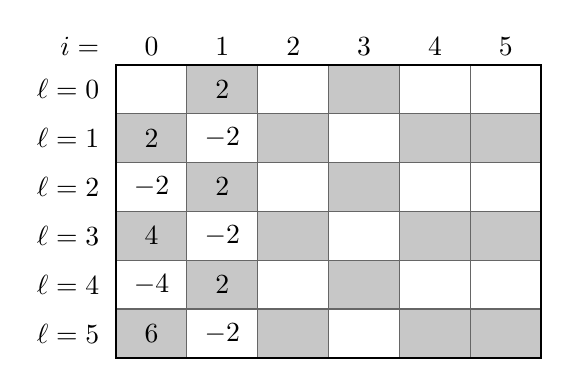
\begin{tikzpicture}[x=0.9cm,y=0.62cm]
  \fill[black!22] (1,0) rectangle (2,1);
  \node at (1.5,0.5) {$2$};
  \fill[black!22] (3,0) rectangle (4,1);
  \fill[black!22] (0,-1) rectangle (1,0);
  \node at (0.5,-0.5) {$2$};
  \node at (1.5,-0.5) {$-2$};
  \fill[black!22] (2,-1) rectangle (3,0);
  \fill[black!22] (4,-1) rectangle (5,0);
  \fill[black!22] (5,-1) rectangle (6,0);
  \node at (0.5,-1.5) {$-2$};
  \fill[black!22] (1,-2) rectangle (2,-1);
  \node at (1.5,-1.5) {$2$};
  \fill[black!22] (3,-2) rectangle (4,-1);
  \fill[black!22] (0,-3) rectangle (1,-2);
  \node at (0.5,-2.5) {$4$};
  \node at (1.5,-2.5) {$-2$};
  \fill[black!22] (2,-3) rectangle (3,-2);
  \fill[black!22] (4,-3) rectangle (5,-2);
  \fill[black!22] (5,-3) rectangle (6,-2);
  \node at (0.5,-3.5) {$-4$};
  \fill[black!22] (1,-4) rectangle (2,-3);
  \node at (1.5,-3.5) {$2$};
  \fill[black!22] (3,-4) rectangle (4,-3);
  \fill[black!22] (0,-5) rectangle (1,-4);
  \node at (0.5,-4.5) {$6$};
  \node at (1.5,-4.5) {$-2$};
  \fill[black!22] (2,-5) rectangle (3,-4);
  \fill[black!22] (4,-5) rectangle (5,-4);
  \fill[black!22] (5,-5) rectangle (6,-4);
  \foreach \x in {1,...,5} \draw[black!60] (\x,-5) -- (\x,1);
  \foreach \y in {-4,...,0} \draw[black!60] (0,\y) -- (6,\y);
  \draw[line width=0.7pt] (0,-5) rectangle (6,1);
  \node[above] at (0.5,1) {$0$};
  \node[above] at (1.5,1) {$1$};
  \node[above] at (2.5,1) {$2$};
  \node[above] at (3.5,1) {$3$};
  \node[above] at (4.5,1) {$4$};
  \node[above] at (5.5,1) {$5$};
  \node[above left] at (-0.1,1) {$i=$};
  \node[left] at (-0.1,0.5) {$\ell=0$};
  \node[left] at (-0.1,-0.5) {$\ell=1$};
  \node[left] at (-0.1,-1.5) {$\ell=2$};
  \node[left] at (-0.1,-2.5) {$\ell=3$};
  \node[left] at (-0.1,-3.5) {$\ell=4$};
  \node[left] at (-0.1,-4.5) {$\ell=5$};
\end{tikzpicture}
\caption{The $\sigma$-bump of the example at $k=6$, with $S=\{1,2,4,5\}$,
$\sigma=1$ and $Q=\{1,3\}$. Row $\ell$ holds the positions $n=6\ell+i$,
$0\le i<6$, so time runs left to right and then down. Shaded cells are the
positions in the anti-periodic set $P$, where the orbit $E$ equals $-1$;
elsewhere $E=0$. Each row is the complement of the one above, so the
pattern repeats every two rows, that is, with period $2k=12$. The numbers
are the nonzero values of the bump $d$ of \eqref{eq:trop-bump}; blank cells
have $d_n=0$. In column $1$ the bump alternates between $2$ and $-2$, while
in column $0$ it grows without bound, $d_{12m}=-2m$. Every negative entry
lies in an unshaded cell, as \eqref{eq:trop-bumpnonneg} requires.}
\label{fig:nao-bump}
\end{figure}
Consequently, by \autoref{thm:sigmabump}, no equation $x_{n+6}x_n=c_0+c_1x_{n+1}
+c_2x_{n+2}+c_4x_{n+4}+c_5x_{n+5}$ with positive $c_1,c_2,c_4,c_5$ is
globally periodic.

\subsection{The mirror}

Let $S\subseteq\{1,\dots,k-1\}$ be palindromic. If $Q$ satisfies (B1) for
$\sigma$, its reflection $Q'=k-Q$ satisfies (B1) for $k-\sigma$, and the
reflection turns a read of $1$ at the index $k-i$ for $(k-\sigma,Q')$ into a
read of $0$ at the index $i$ for $(\sigma,Q)$. This halves the work: to check
(B2) for $(\sigma,Q)$ it is enough to find a surviving tap reading $1$ at
every index, both for $(\sigma,Q)$ and for $(k-\sigma,Q')$.

\begin{lemma}[the mirror]
\label{lem:nao-mirror}
Let $S$ be palindromic, $\sigma\in S$, and let $Q,Q'\subseteq\{1,\dots,k-1\}$
satisfy $y\in Q'\iff k-y\in Q$ for $0<y<k$. If at the index $k-i$ the tap
$j'$ survives for $(k-\sigma,Q')$ and reads $v$, then at the index $i$ the tap
$k-j'$ survives for $(\sigma,Q)$ and reads $1-v$.
\end{lemma}

\begin{proof}
Let $P$ and $P'$ be the anti-periodic sets of $Q$ and $Q'$. The tap $k-j'$
lies in $S$ by palindromy. At $i$ it reads the position $p=i+k-j'$, and at
$k-i$ the tap $j'$ reads the position $p'=k-i+j'$, so $p+p'=2k$. Hence
$p\equiv-p'\pmod k$, and since $\sigma\equiv-(k-\sigma)$, the tap $k-j'$ is
deleted at $i$ exactly when $j'$ is deleted at $k-i$. For the reads, let
$r=p'\bmod k$, which is nonzero as $j'$ survives. If $p'=r$, then
$p=(k-r)+k$, so by \eqref{eq:read-antiper}
$p\in P\iff k-r\notin Q\iff r\notin Q'\iff p'\notin P'$. If $p'=r+k$, then
$p=k-r$ and $p\in P\iff k-r\in Q\iff r\in Q'\iff p'\notin P'$. Either way
the two reads are complementary.
\end{proof}
